\chapter{Caso di studio}
Con l'evolversi della tecnologia, ed in particolare con l'avvento dell'IoT,
l'aspettativa delle applicazioni basate sul cloud è cambiata. La necessità di
elaborare un numero sempre maggiore di dati ha spinto, sempre più aziende, ad
adottare strumenti cloud based forniti da terzi come ad esempio Microsoft Azure o Amazon
AWS.  Ed è utilizzando questi servizi  che l'architettura classica del
software monolitico ha mostrato i suoi limiti. Con architettura monolitica si
intende una applicazione self-contained indipendente dalle altre
applicazioni presenti nel sistema.  Basandosi su questa modello, ogni
software necessita di essere disinstallato e reinstallato nel momento in cui
sia necessario apportare delle semplici modifiche. Per superare i limiti del
modello monolitico, è stato introdotto il concetto di 
\emph{microservzio}.  La differenza tra una architettura monolitica ed una
basata su microservizi è la  modularità che quest'ultima garantisce.  Prendiamo
come esempio una applicazione formata da un database, un interfaccia web
(client-side user interface)  e una applicazione server (server-side
application).  L'applicazione server-side interpreterà le richieste fatte
dall'utente andando ad eseguire operazioni interne al server, aggiornerà il
database e fornirà il risultato all'utente finale tramite l'interfaccia web.
Nel modello classico  è necessario riscrivere o aggiornare l'intero 
software per apportare delle modifiche o aggiungere delle funzionalità.\\ 
Con il termine \emph{microservices}
si intende una architettura basata su oggetti chiamati \emph{component} ognuno
dei quali fornisce ed utilizza dei \emph{servizi}. Con \textit{component}, si intende
una "parte" di software che può essere aggiornata e sostituita indipendente
dalla applicazione principale.  Ogni \emph{component} si basa sull'utilizzo e la
condivisione di servizi.  I servizi sono l'equivalente delle librerie in una
architettura monolitica, al contrario di queste ultime però, i servizi sono
sviluppabili indipendentemente dalla applicazione principale.
In questo capitolo verrà esposto lo sviluppo di due 
 di applicativi per la gestione e l'interazione di sensori
basti su LoRa, tramite l'utilizzo del framework EveryWare Software Framework ESF
basato su OSGi e sviluppato da Eurotech.
\section{OSGi}
La tecnologia OSGi (Open Services Gateway initiative),
è un insieme di specifiche che definiscono dei componenti
dinamici in grado di estendere le funzionalità dell'ambiente  Java.
Basandosi su di una architettura a microservizi, OSGi permette la gestione in
modo remoto di componenti chiamati Bundle o Deployment Package(dp), i quali
possono essere installati, attivati, aggiornati e fermati senza la necessità di
riavviare l'applicazione principale\\
Ogni bundle è composto dai file contenti le classi ed i metodi specifici per le
funzionalità che implementa e da  metadati utili al framework
per distinguere le classi private da quelle pubbliche. 
Per rendere compatibile questa architettura con il linguaggio di programmazione
Java e la Java Virtual Machine, OSGi ha strutturato il framework su vari
livelli:
\begin{itemize}
        \item   \textit{Bundles}. Bundles sono normali applicazioni JAR contenenti
        \item   \textit{Services}. Il service layer connette in maniera dinamica
                i bundles offrendo un modello publish-find-bind basto su
                l'interfaccia Java POJIs.
        \item   \textit{Services Registry}. Questo layer è composto da una serie
                 API per la gestione dei servizi.
        \item   \textit{Life-Cycle}. Insieme di API per gestire \hyperlink{cycle_bundle}{il ciclo vitale
                dei bundle}
        \item   \textit{Modules}. È il layer che definisce in che modo i bundle
                sono in grado di interagire importando ed esportando pezzi di
                codice.
        \item   \textit{Security} È un layer che opera su tutti i livelli e
                garantisce la sicurezza delle applicazioni OSGi andando a
                limitare le funzionalità del bundle.
\end{itemize}
\begin{figure}[th]
\centering 
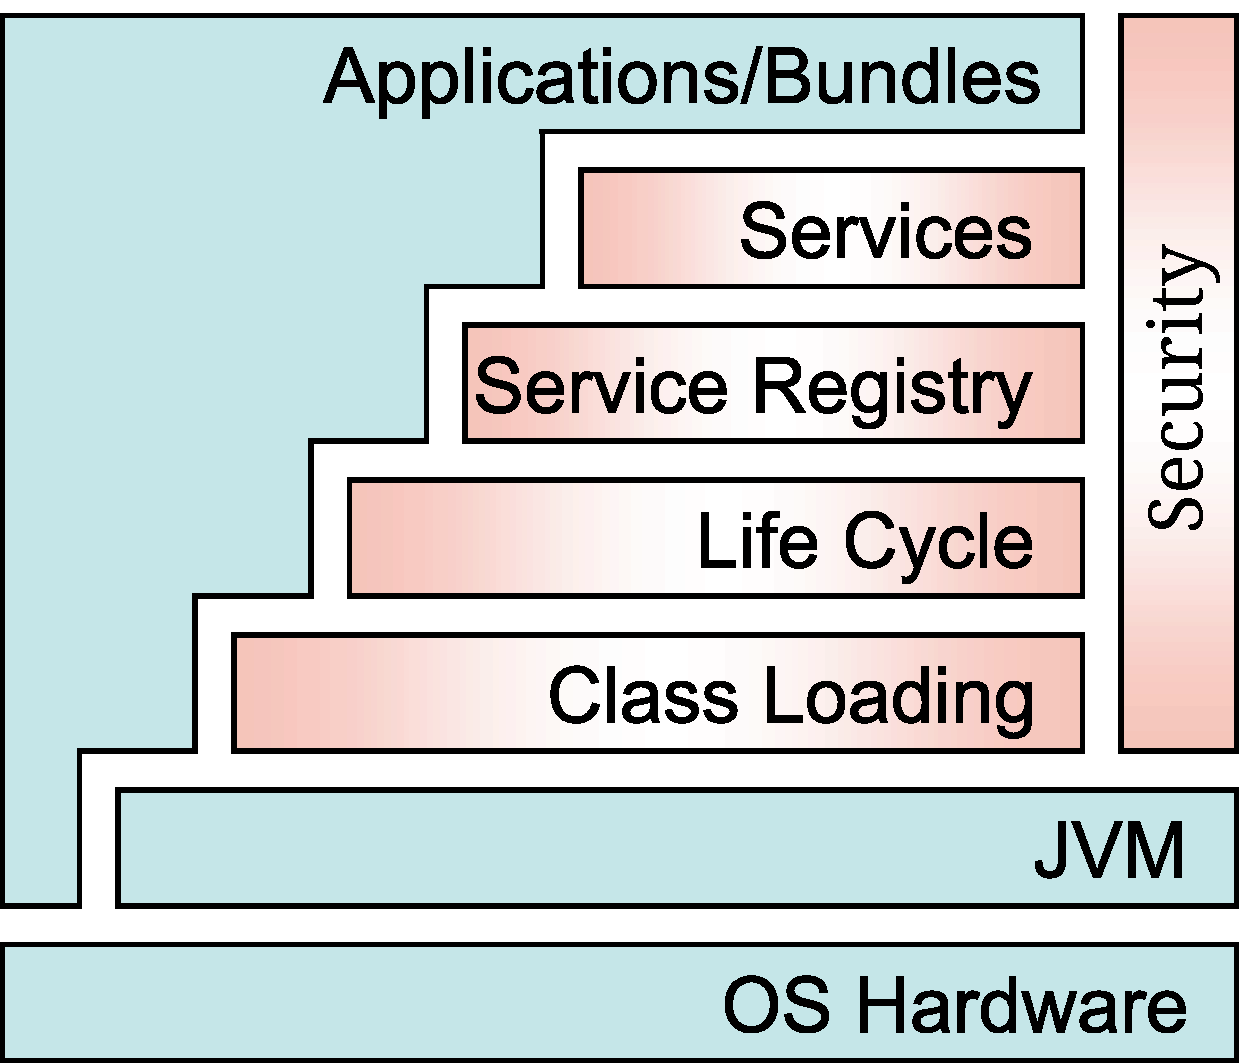
\includegraphics[width=10cm]{osgi}
\caption{Layer OSGi}
\label{}
\end{figure}

\subsection{Ciclo vitale dei bundle}\hypertarget{cycle_bundle}{}
In un modello così dinamico, è necessario che il framework sia basato su di un
software fail-safe in grado di gestire le eccezioni che si possono verificare
durante l'installazione e disinstallazione di nuovi moduli.
Non è raro infatti che nuovi bundle ,installati nel sistema, richiedano servizi
non ancora disponibili o attualmente utilizzati da altri componenti.
Per far fronte ai problemi riscontrabili, OSGi assegna ad ogni  i bundle  uno 
\emph{stato} tra:
\begin{itemize}
        \item   \textit{Installed} Il bundle è stato installato nel sistema, ma
                non sono presenti alcune delle sue dipendenze.
        \item   \textit{Resolved} Il bundle è installato e le sue dipendenze
                presenti nel sistema.
        \item   \textit{Starting} Uno stadio temporaneo attraverso il quale il
                bundle passa prima di essere attivato.
        \item   \textit{Active} Il bundle è stato correttamente attivato e sta
                eseguendo le sue funzioni all'interno del sistema.
        \item   \textit{Stopping} Uno stadio temporaneo in cui il bundle passa
                prima di essere disattivato.
        \item   \textit{Uninstalled} Il bundle è stato rimosso dal container
                OSGi
\end{itemize}

\subsection{Module layer}
Il module layer è dove il framework OSGi gestisce la "modularità" di un bundle.
È in questo layer che vengono processati i metadati contenuti all'interno del
file MANIFEST.MF. Tramite questo file il framework OSGi è in grado di
determinare le dipendenze del bundle e quali servizi è in grado di esportare.

\subsection{Registrazione del servizio}
Un \emph{servizio} in OSGi è definito tramite una classe Java standard. Per
implementare un nuovo servizio, è necessario definire quale classe o quale
interfaccia si vuole fornire il servizio.
La soluzione a questo, è l'utilizzo di registri di servizio. Ogni bundle può
esporre dei metodi ed registrarli attraverso il service registry. In questo
modo, altri bundle possono accedere al service registry e utilizzare i metodi
listati nel registro. Un bundle quindi può registrare un servizio, può
utilizzare un servizio oppure può mettersi in attesa aspettando che un servizio
venga registrato o eliminato.
Inoltre i servizi sono dinamici, ogni bundle può mettersi in lista per
richiedere un servizio mentre altri stanno ancora utilizzando il servizio.
\begin{figure}[th]
        \centering 
                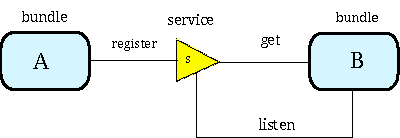
\includegraphics[width=9cm]{osgi_service}
        \caption{Schema utilizzo servizi OSGi}
        \label{}
\end{figure}

\section{Everyware Software}
ESF o Everyware Software è un framework che si interpone tra il sistema operativo
e le applicazioni utente. Basato su Java/OSGi, ESF si pone l'obiettivo di
offrire  la possibilità di sviluppare applicativi, per il mercato M2M ,in maniera semplice e veloce
. Ideato per operare all'interno di gateway
industriali, fornisce al consumatore servizi e librerie per l'accesso delle più
comuni porte di comunicazione RS232/485, GPIO, CAN.
ESF tramite la sua interfaccia web, permette di controllare da remoto il
comportamento dei gatway.
\ref{fig:ESF_web}.
%\begin{figure}[th]
%        \centering 
%                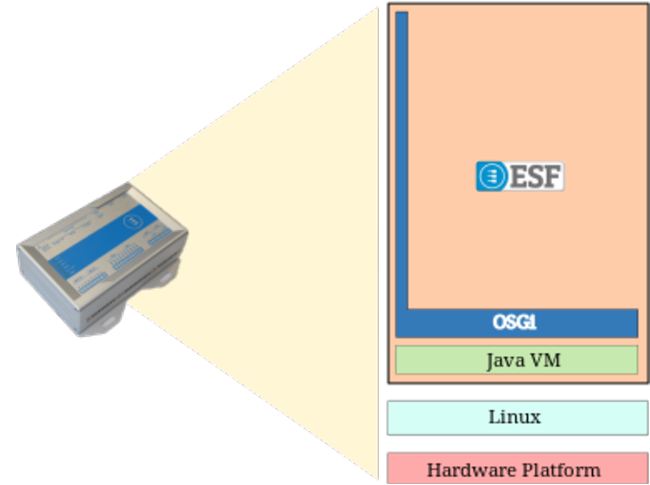
\includegraphics[width=10cm]{ESF_layer.pdf}
%        \caption{OSGi services}
%        \label{}
%\end{figure}


\begin{figure}[th]
        \centering 
                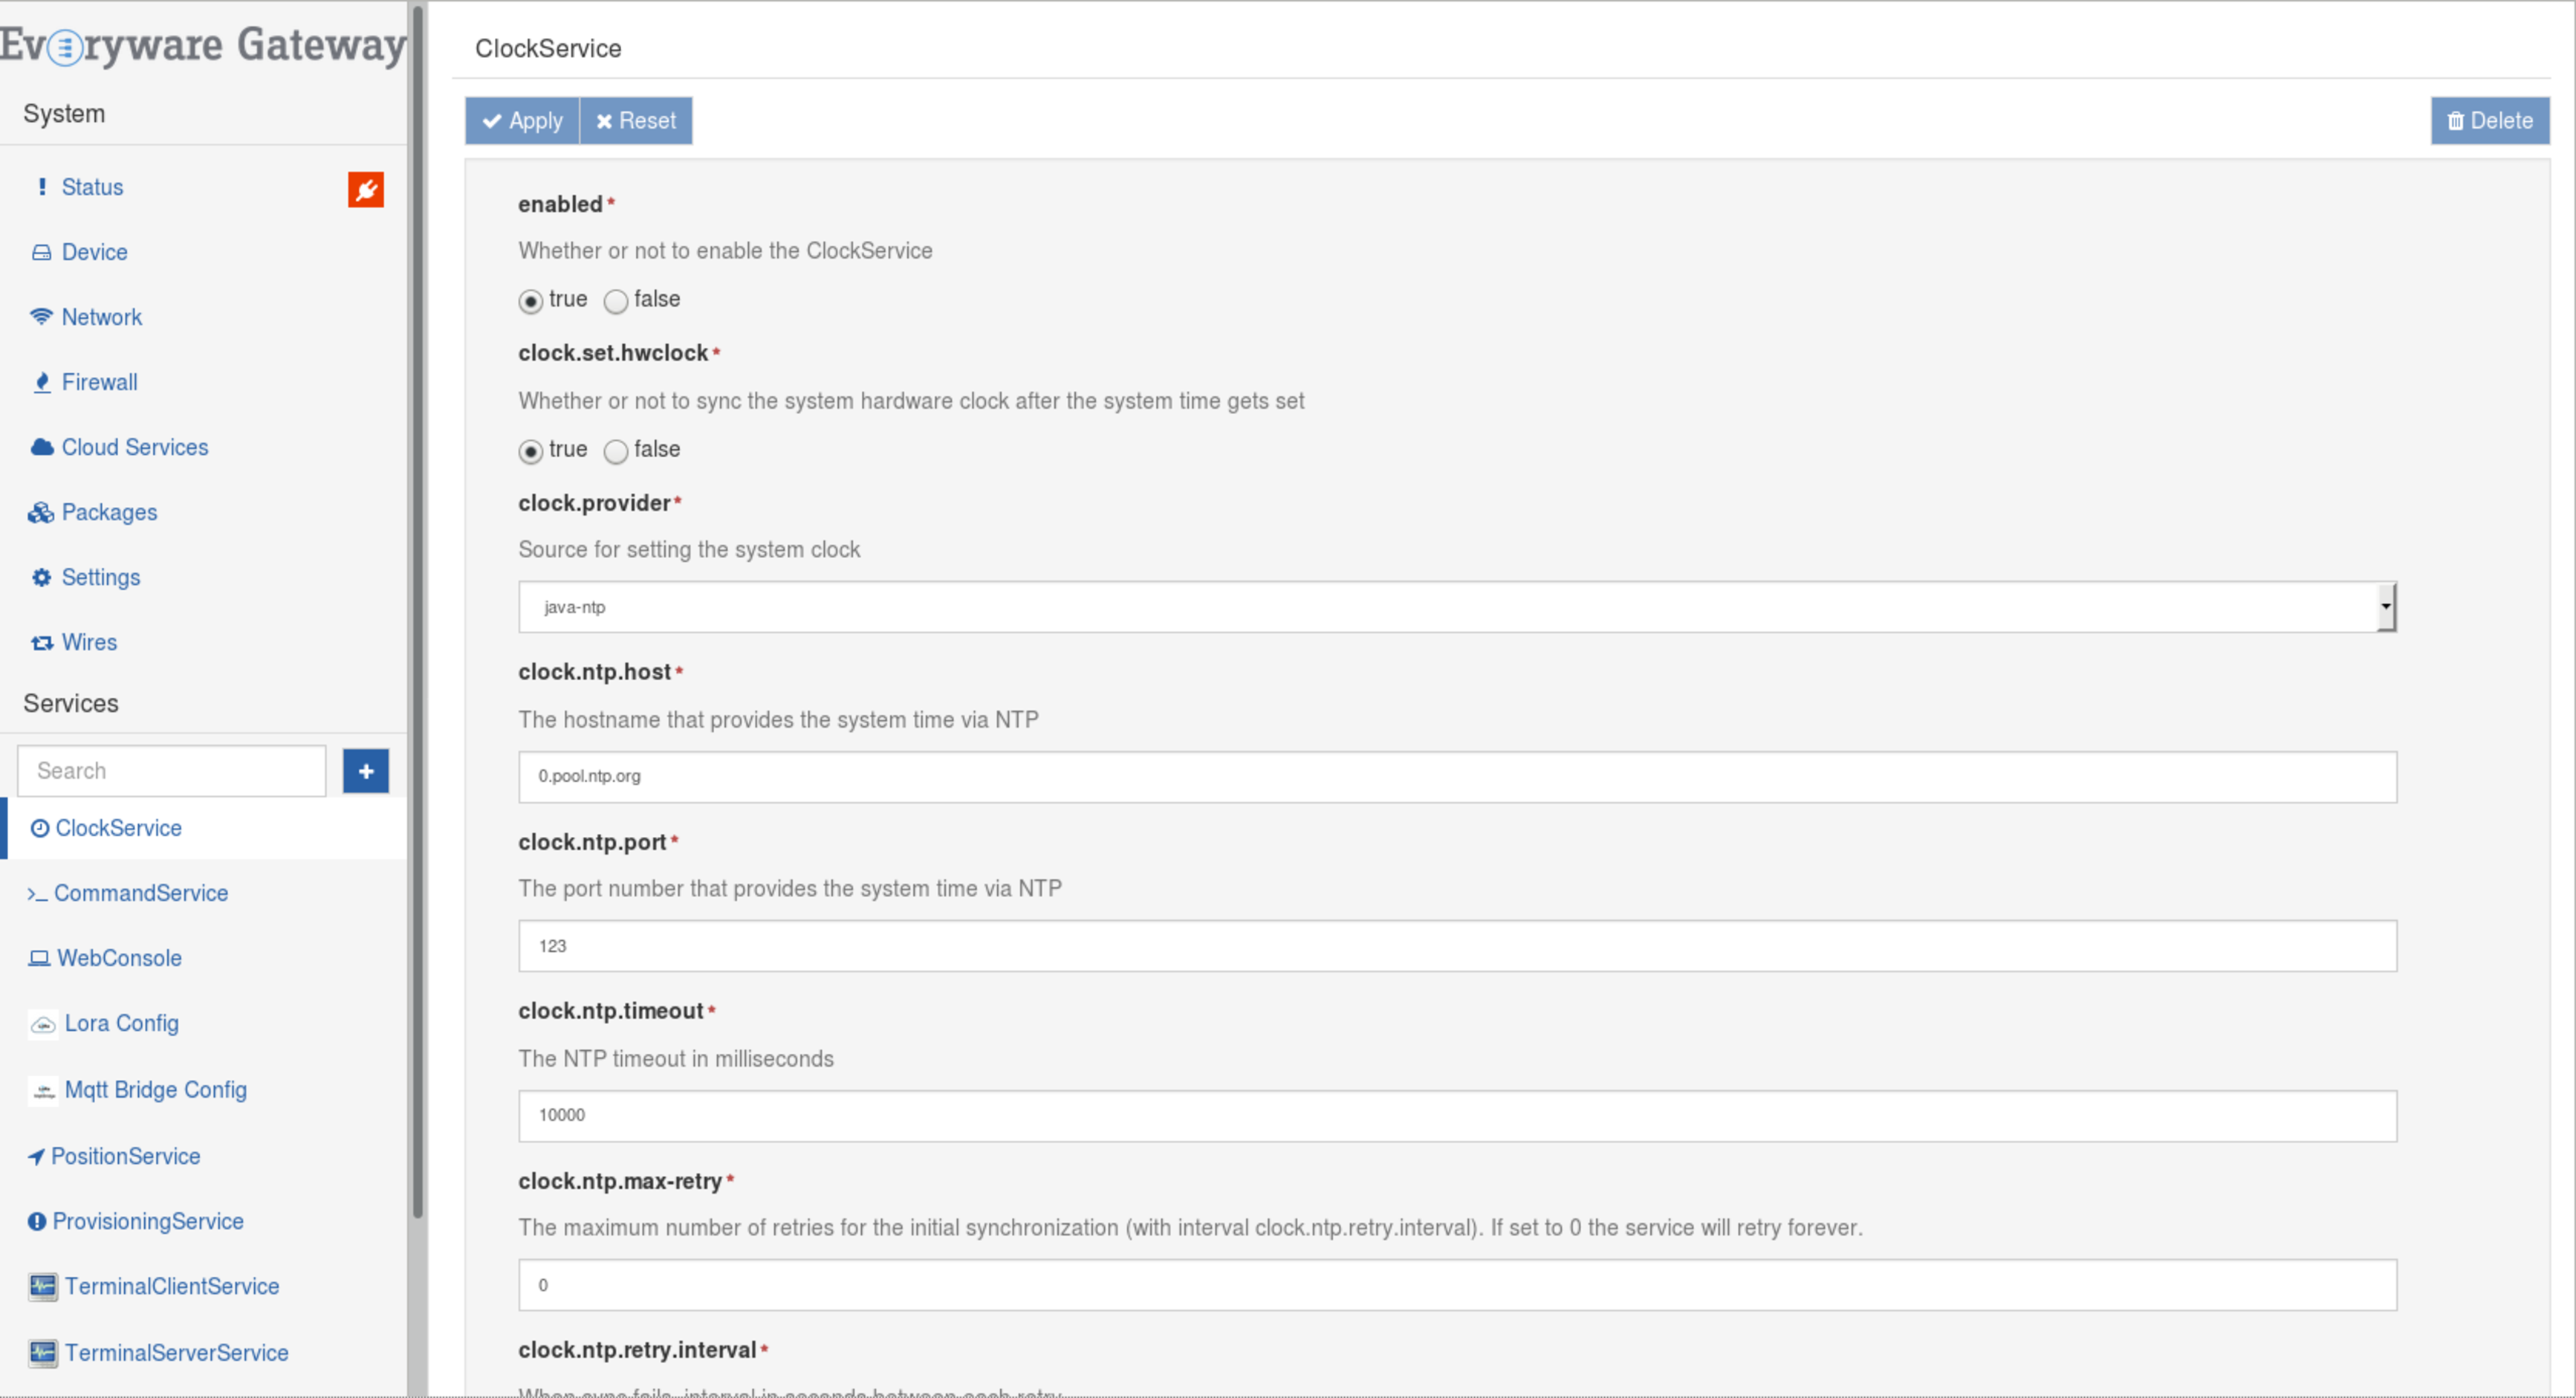
\includegraphics[width=12cm]{ESF.png}
                \caption{Interfaccia web ESF}
        \label{fig:ESF_web}
\end{figure}

\pagebreak


\section{Architettura del software}
Per integrare ESF con il ricevitore lora SX1301, è stato necessario l'utilizzo
di due software aggiuntivi.
Il primo è LoRa packet forwarder fornito da Semtech. Questo
applicativo permette di comunicare con le periferiche di basso livello presenti
nel ReliaGATE 10-11 in modo da astrarre ad un più alto livello i dati ricevuti dal
ricevitore .
L'altra applicazione utilizzata, è LoRa Gateway Bridge. Tramite questa
applicazione è stato possibile 
reindirizzare i dei dati forniti dal packet forwarder ad un server MQTT.

\begin{figure}[th]
        \centering 
                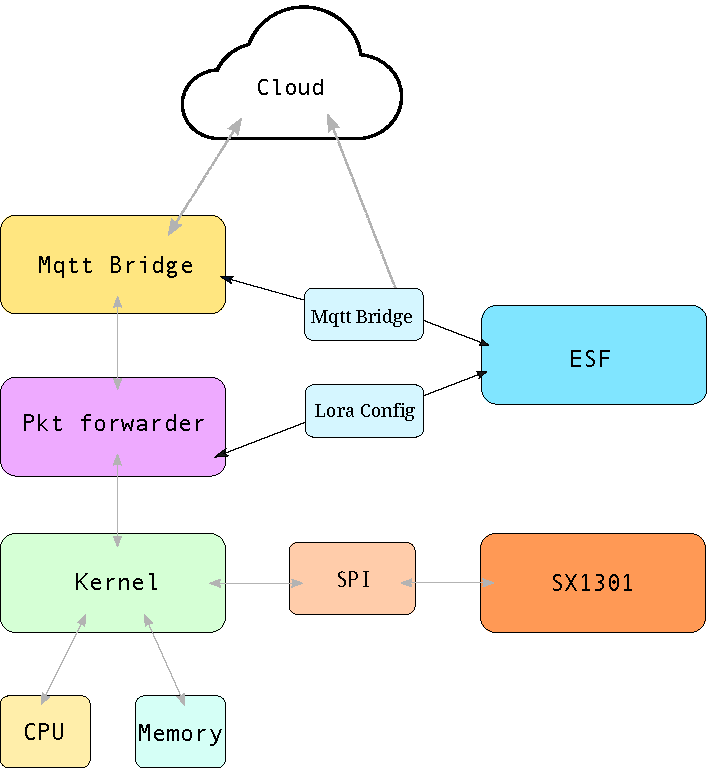
\includegraphics[width=11cm]{Application_layer}
        \caption{Architettura del software}
        \label{fig:Software_stack}
\end{figure}

\subsection{Semtech packet forwarder}
Il packet forwarder è un software che permette la ricezione e l'invio di pacchetti radio Lora ,
tramite una connessione SPI con il device SX1301. Nel caso di ricezione di un
pacchetto, l'applicativo incapsula i dati ricevuti in un formato UDP, e li
ritrasmette nella rete internet/intranet. Per la sua configurazione viene
utilizzato un file Json nel quale troviamo tutte le varie opzioni di
configurazione per i moduli radio presenti al interno del chip.
\inputminted[mathescape, gobble=2, frame=lines, linenos=true
framesep=2mm, firstline=1,lastline=23]{json}{Code_Files/global_json.conf}
\inputminted[mathescape, gobble=2, frame=lines, linenos=true
framesep=2mm, firstline=173,lastline=184]{json}{Code_Files/global_json.conf}

\subsection{LoRa Gateway Bridge}
LoRa Gateway Bridge è un applicativo in grado di identificare i vari pachetti UDP inviati
dal packet forwarder e inotrarli ad un Broker MQTT. 
Il software è scritto nel linguaggio GO e permette una configurazione tramite
linea di comando.  Per renderlo interfaciabile con ESF, sono state apportate delle 
modifiche al codice; in particolare è stata aggiunta la possibilità di
specificare il publish e il subscribed topic, i quali erano hard-coded.
%\inputminted[mathescape, gobble=2, frame=lines, linenos=true
%framesep=2mm, firstline=1,lastline=23]{go}{Code_Files/bridge_mqtt.go}
Il codice sottostante, rappresenta un esempio di pacchetto LoRa inoltrato dal
LoRa Gateway Bridge ad un broker MQTT
\inputminted[mathescape, gobble=2, frame=lines, linenos=true
framesep=2mm, firstline=1,lastline=23]{json}{Code_Files/message.json}
\section{Hardware utilizzato}

\subsection{SX1301}
Per la ricezione dei pacchetti LoRa, è stato utilizzato il chip SX1301 prodotto
da Semtech e collegato al gateway ReliaGate 10-11.
\subsubsection{Struttura interna}
Per quanto riguarda la struttura interna del modulo radio, non si hanno molte
informazioni dato che la tecnologia è proprietaria di Semtech. Nella
documentazione ufficiale è presente una rappresentazione grafica dei vari
blocchi interni al chip.

\begin{figure}[th]
        \centering 
                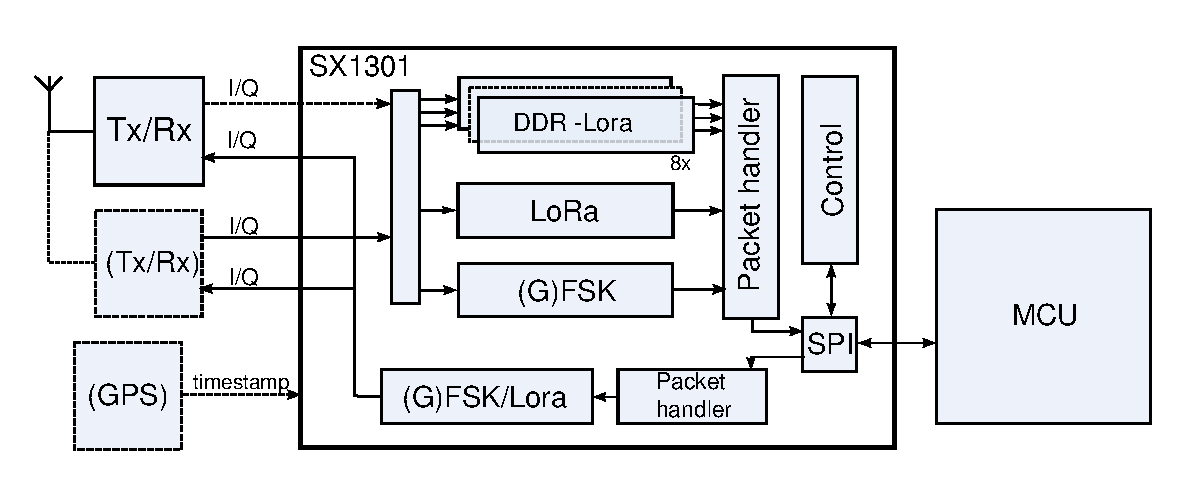
\includegraphics[width=11cm]{SX1301}
        \caption{Struttura interna ricevitore SX1301}
        \label{fig:sx1301}
\end{figure}

Come scritto nella documentazione  \improvement{inserire link} e intuibile dalla
figura \ref{fig:sx1301} il chip è in grado di scansionare contemporaneamente 
8 canali diversi (IF0 a IF7)  permettendoli di rimanere in ascolto per garantire
la ricezione dei segnali con SF diversi.
Inoltre data la quasi ortogonalità degli Spreading Factor
, il chip è in grado di ricevere un pacchetto
con uno Spreading Factor $i$ anche nel caso in cui si sovrapponga ad un altro
pacchetto con Spreading Factor pari a $j$, fintanto che $i\neq j$. Questa
pseudo-ortogonalità utilizzata in LoRa, permette al ricevitore  SX1301 
di demodulare fino ad un massimo di 8 pacchetti contemporaneamente.
Nella tabella \ref{tab:sx1301_spec} sono riportate le caratteristiche elettriche
massime del  chip SX1301. Il Chip, supporta tensioni di
alimentazione fino a 4V e  come e possibile osservare il range di temperatura in cui il
chip può operare è molto ampio, rendendolo ideale per applicazioni esterne ed
interne. 

\begin{table}[th]
        \centering 
                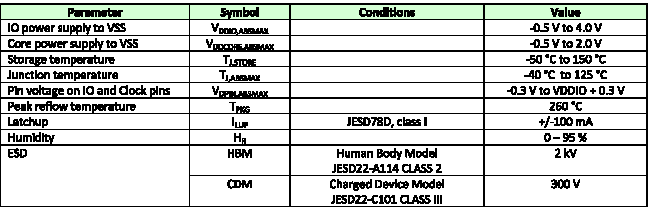
\includegraphics[width=16cm]{SX1301_table}
        \caption{Caratteristiche elettriche SX1301}
\label{tab:sx1301_spec}
\end{table}
Utilizzando i valori nominali riportati nella tabella \ref{tab:sx1301_spec_1},
si hanno valori di corrente pari a 1[uA] in idle  e di 5[mA] in pieno
funzionamento.
\begin{table}[th]
        \centering 
                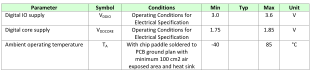
\includegraphics[width=16cm]{SX1301_table_1}
        \caption{Caratteristiche elettriche SX1301}
        \label{tab:sx1301_spec_1}
\end{table}
Per la ricezione del segnale è stata utlizzata una antenna omnidirezionale,
ideata per la banda degli 868[MHz] con un guadagno pari a 3[dB].
\subsection{ReliaGATE}
Il gateway a cui è collegato il modulo SX1301 è il ReliaGATE 10-11 prodotto da
Eurotech. Al suo interno troviamo un processore Texas Instruments TI AM335X Cortex-A8 
equipaggiato con 512MB di RAM e 4GB di storage eMMC. Il ReliaGATE offre una
vasta gamma di porte tra cui 232/485, 2CAN bus, 2 porte USB e 2 porte Ethernet,
inoltre ha connettività Bluetooth, WiFi e GPS. Al suo interno è installo
Everyware™ Software Framework (ESF) versione 5.
\begin{figure}[th]
        \centering 
                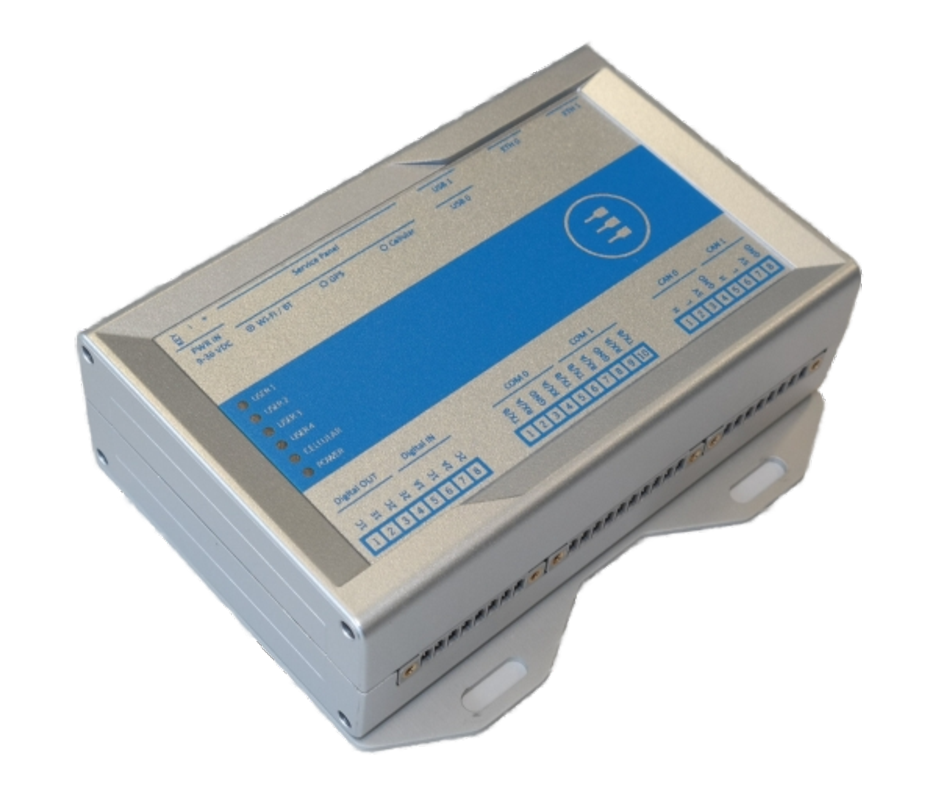
\includegraphics[width=11cm]{Reliagate_10_11}
        \caption{ReliaGATE 10-11}
        \label{fig:ReliaGATE}
\end{figure}



\section{Realizzazione}

Per gestire i due software preinstallati si è optato per la creazione di due
applicativi osgi distinti Lora Config e Mqtt Bridge.
\subsection{Lora Config}
Il primo applicativo chiamato Lora Config si pone il compito di leggere ed
interpretare il file di configurazione utilizzato dal programma \emph{Packet
Forwarder}, per poi andare ad esporre i parametri principali all'utente tramite
l'interfaccia web di ESF.
La libreria utilizzata per manipolare i file di tipo Json è 

\mint{Java}|import com.eclipsesource.json|

Tramite la quale vengono riempiti i campi della classe LoraSettings. Il file
Json è composto da due parti. Nella prima parte
troviamo tutte le impostazioni per la configurazione dei canali (IF0 a IF7)
, nella seconda
parte sono presenti le impostazioni per il forward dei pacchetti. 
Per semplificare la gestione del bundle, sono state create due classi distinte
SX1301Configuration e GatewayConfiguration, accessibili tramite la classe LoraSettings.

\begin{minted}[linenos=true, numbersep=5pt, gobble=2, frame=lines, %
framesep=2mm]{java}
    public class LoraSettings {
            public static final String KEY_GATEWAY_CONFIG = "gateway_conf";
            public static final String KEY_SX1301 = "SX1301_conf";
            private SX1301Configuration sx1301Conf;
            private GatewayConfiguration gatewayConf;
       } 
\end{minted}

Per applicare le modifiche apportate alla configurazione, è necessario che
il packet forwarder venga riavviato. Per eseguire questa operazione si è scelto di
utilizzare la libreria 
\mint{Java}|import com.apache.commons.exec|
la quale fornisce delle API per chiamare processi esterni, in particolare
si è scelto di utilizzare l'utility di sistema \emph{pkill} per terminare il
processo del pkt forwarder.
\begin{minted}[linenos=true, numbersep=5pt, gobble=2, frame=lines, %
framesep=2mm]{java}
          public void startPktForwarder() {
                DefaultExecutor pktExecutor = new DefaultExecutor();
                CommandLine pktCmdLine = new CommandLine(KEY_PKT_BIN);
                pktCmdLine.addArgument("start");
                pktExecutor.setExitValue(0);
                try {

                    pktExecutor.execute(pktCmdLine);
                    s_logger.info("start PKT");
                } catch (Exception e) {
                    s_logger.warn("Coulden't start pkt forwarder");
                }
            }

            public void stopPktForwarder() {
                DefaultExecutor pktExecutor = new DefaultExecutor();
                CommandLine pktCmdLine = new CommandLine("pkill");
                pktCmdLine.addArgument("basic_pkt_fwd");
                pktExecutor.setExitValue(0);
                try {

                    pktExecutor.execute(pktCmdLine);
                    s_logger.info("Stop PKT");
                } catch (Exception e) {
                    s_logger.warn("Coulden't stop pkt forwarder");
                }
        }

\end{minted}

%\begin{figure}[th]
%        \centering 
%        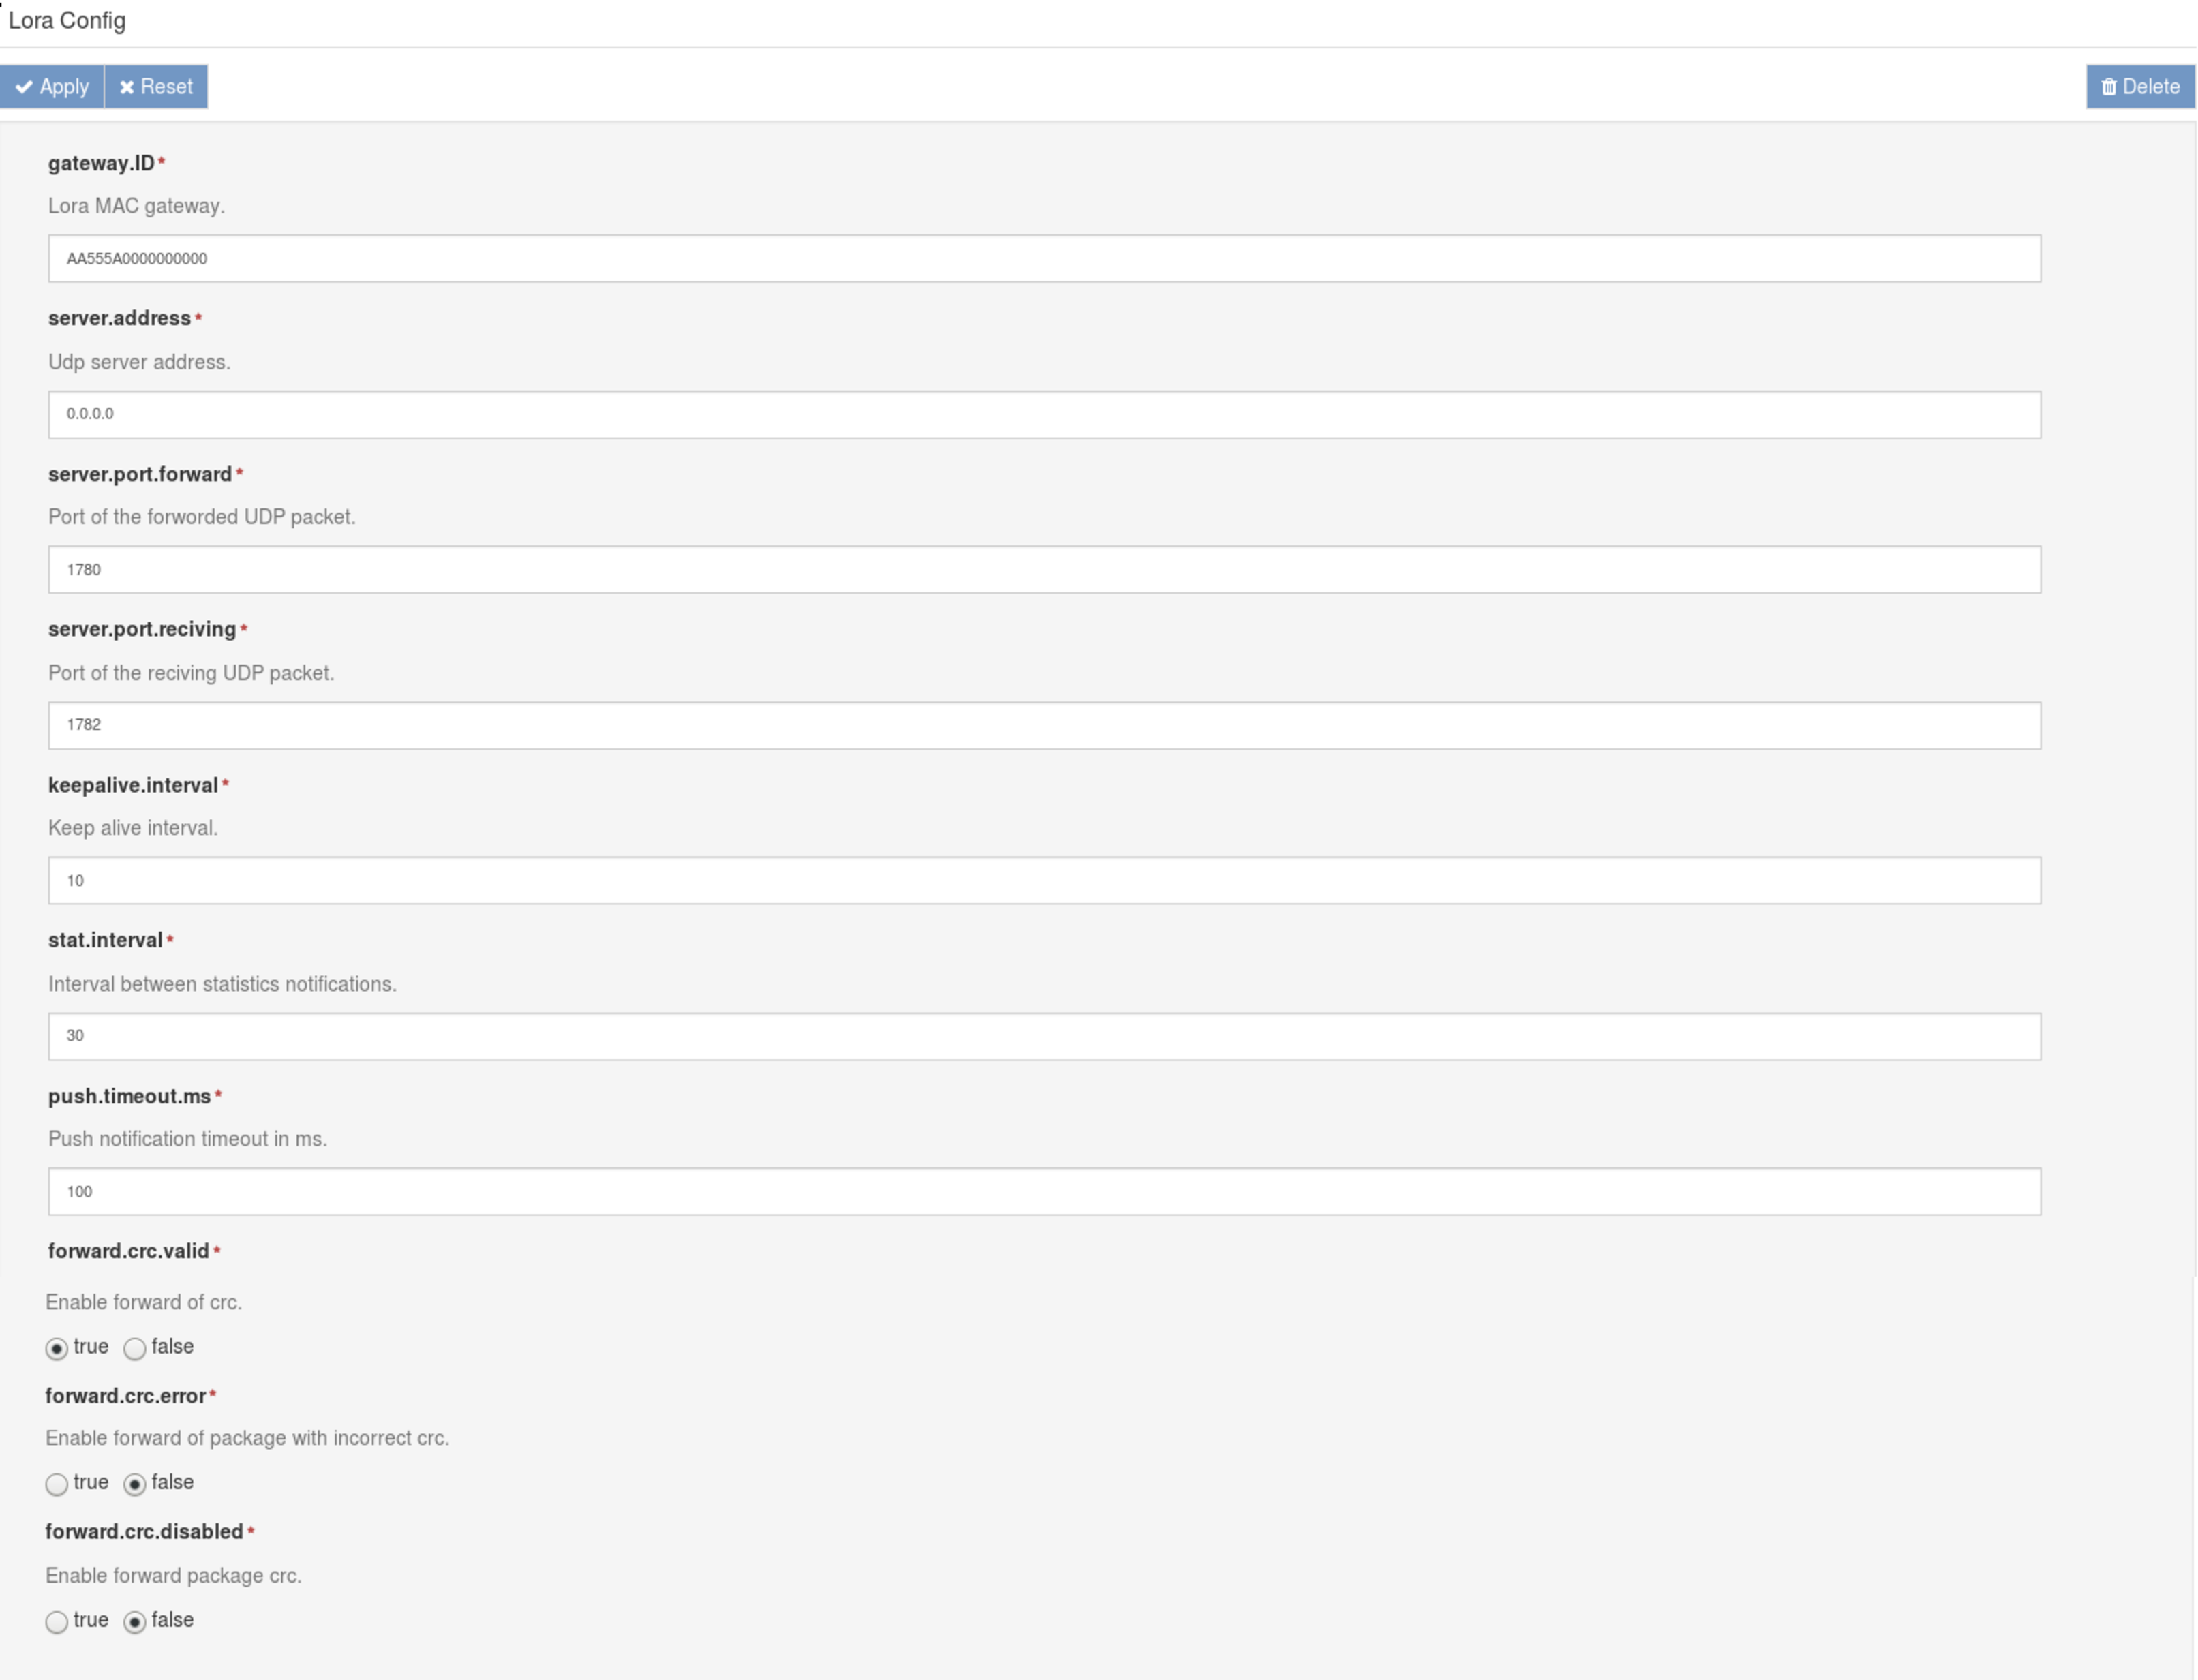
\includegraphics[width=16cm]{Lora_Config}
%                \caption{Architettura del software}
%        \label{fig:Software_stack}
%\end{figure}



\subsection{Mqtt Bridge Config}
Il secondo bundle prende il nome di MQTT Bridge Config e ha lo scopo 
di esporre , tramite l'interfaccia web di ESF, le varie opzioni a linea di
comando dell'applicativo
 \emph{Lora Gateway Bridge}.  Anche in questo caso è necessario il
riavvio del applicativo per fare in modo che le modifiche abbiano effetto. 
Come nel bundle precedente è stata usata la libreria

\mint{Java}|import com.apache.commons.exec|

Tramite l'interfaccia web è possibile modificare i seguenti parametri:
\begin{itemize}
\item il topic sul quale pubblicare i messaggi ricevuti in formato UDP dal
\emph{pkt forwarder}.
\item il topic al quale rimanere il gateway dovrà rimanere in ascolto .
\item su quale indirizzo e porta mandare/ricevere i pacchetti UDP.
\item a quale broker MQTT iscriversi.
\item l'username e password per connettersi al broker.
\end{itemize}

%\begin{figure}[th]
%        \centering 
%                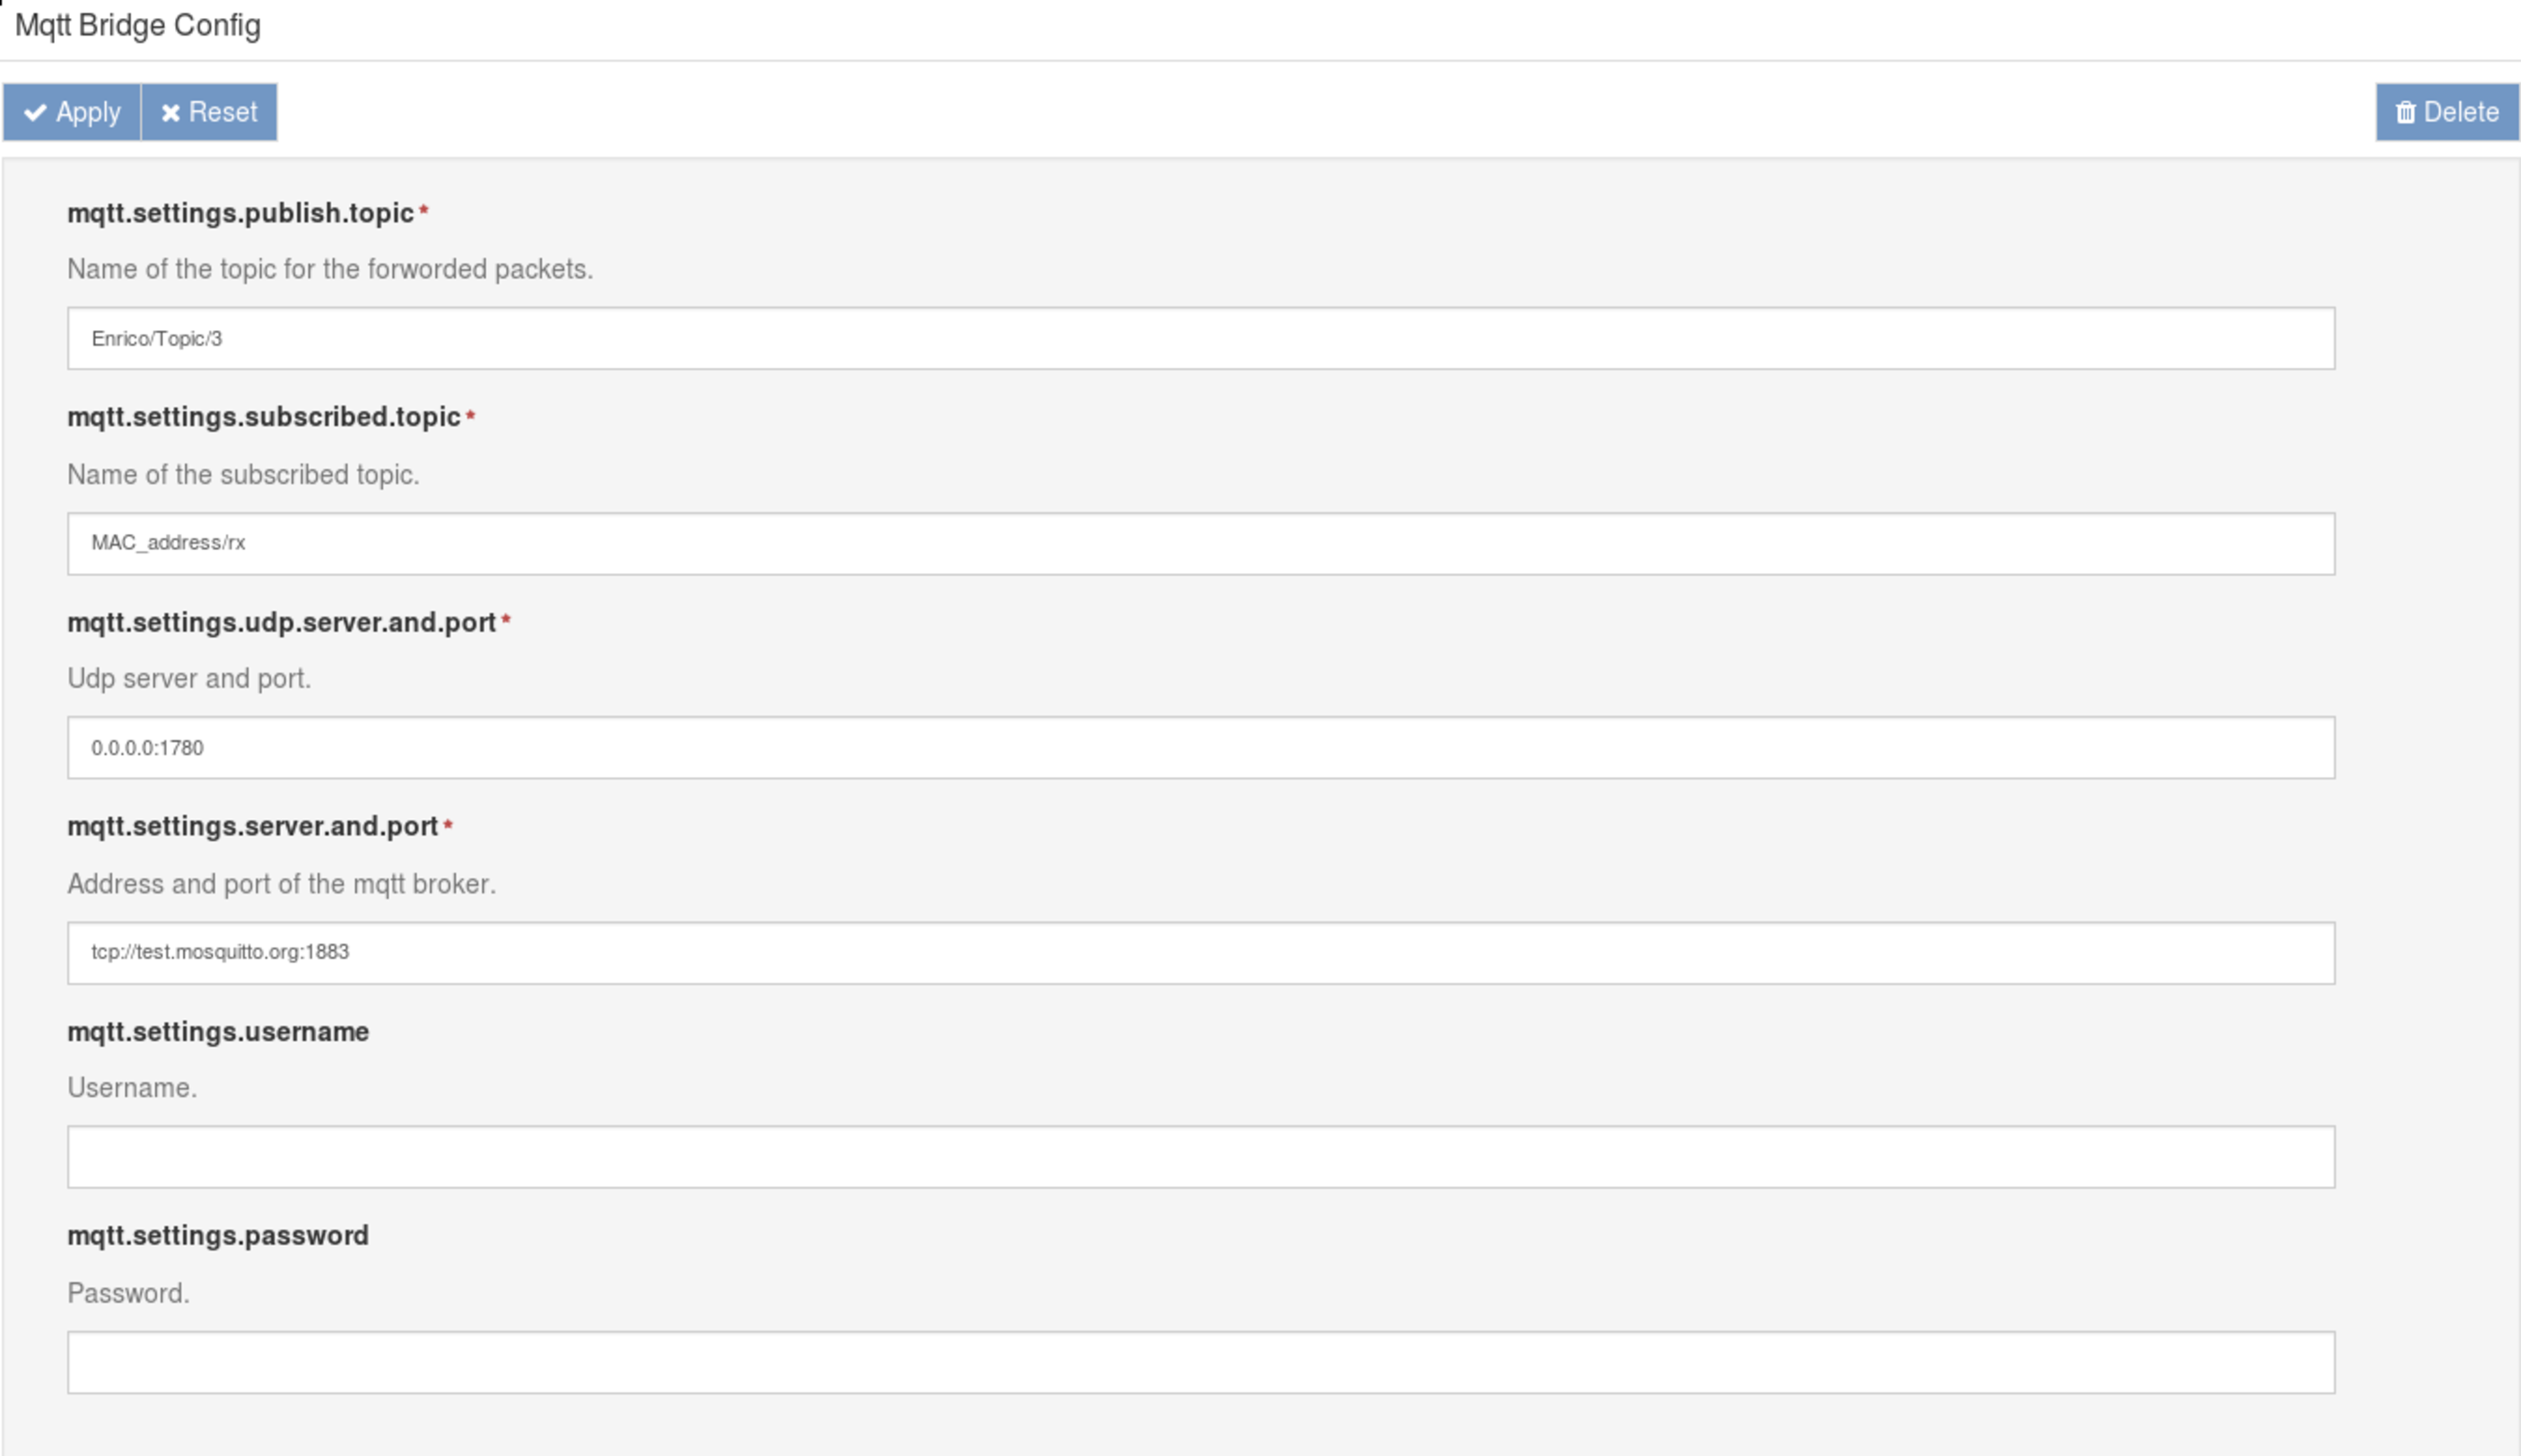
\includegraphics[width=16cm]{Mqtt_Bridge_Config}
%        \caption{Architettura del software}
%        \label{fig:Software_stack}
%\end{figure}

\section{Misurazioni}
Finito lo sviluppo dei bundle, si è scelto di testare la distanza massima
di comunicazione raggiungibile dall'hardware in possesso. 
Il device utilizzato per l'invio dei pacchetti LoRa è prodotto dalla Semtech e
prende il nome di LoRa Mote.
\begin{figure}[th]
        \centering 
                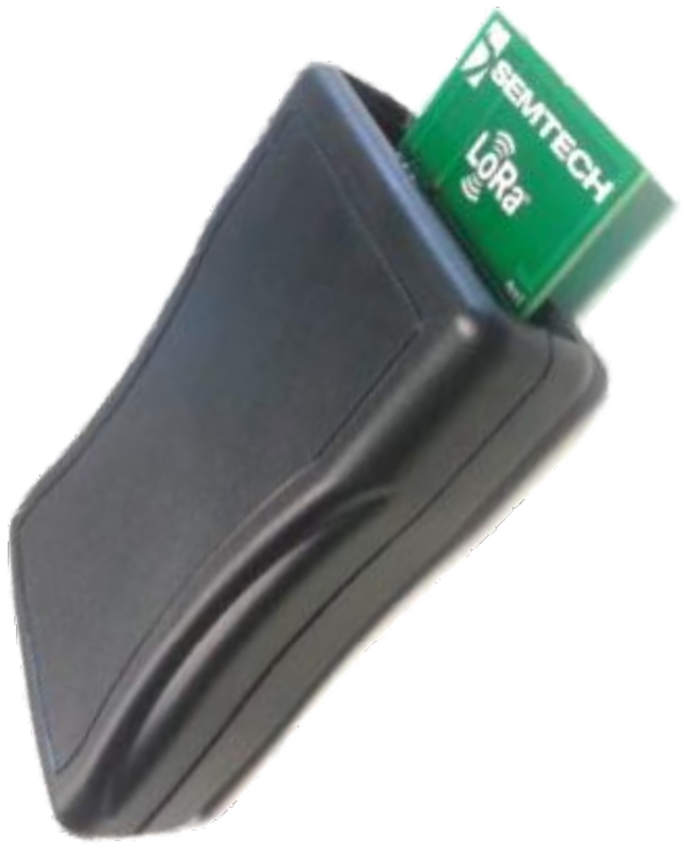
\includegraphics[width=4cm]{LoRaMote_no_wave}
        \caption{Dispositivo LoRa Mote}
        \label{fig:Software_stack}
\end{figure}
In via sperimentale è stato installato  il gateway
ReliaGATE 10-11 ad una altezza di circa 11m. La prova di ricezione è stata condotta per
tentativi cercando , per quanto possibile, di testare diversi punti distribuiti
alla stessa distanza radiale. 
\begin{figure}[th]
        \centering 
                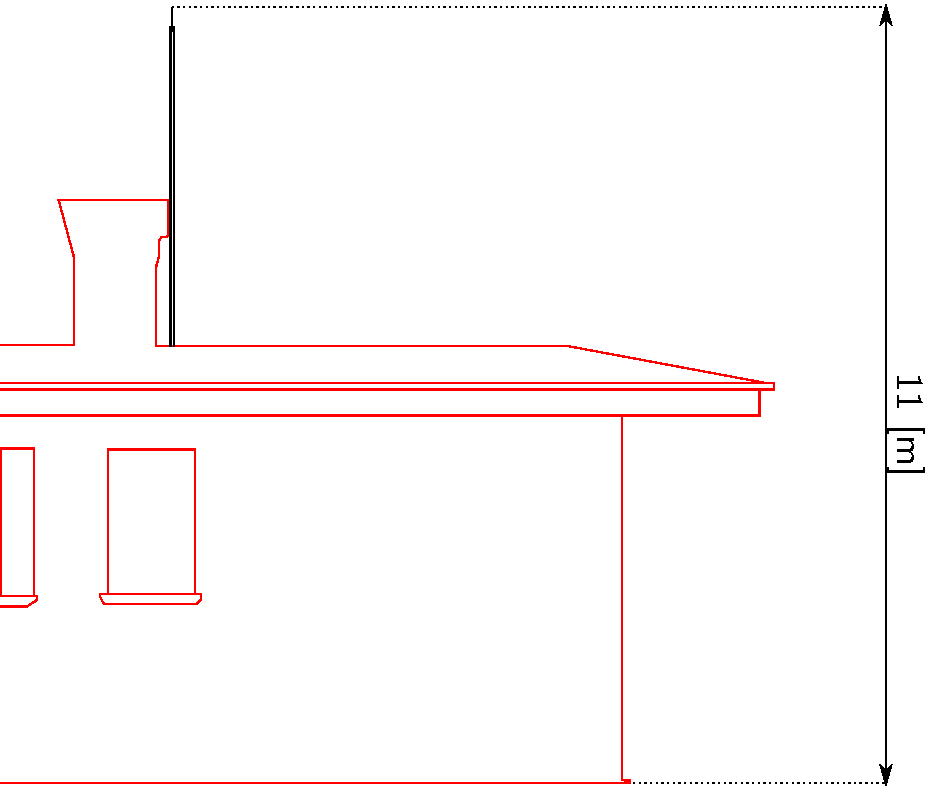
\includegraphics[width=10cm]{casa}
        \caption{Installazione dell'antenna}
        \label{fig:Software_stack}
\end{figure}
Per constatare l'avvenuta ricezione del
messaggio è stata utilizzata l'applicazione Android gratuita \href{
https://play.google.com/store/apps/details?id=at.tripwire.mqtt.client&hl=en}{My
MQTT}, tramite la
quale è possibile iscriversi ad un topic predefinito ed rimanere in ascolto dei
messaggi pubblicati in esso. 
Come broker MQTT si è scelto di utilizzare il
broker open source \href{http://mosquitto.org/}{"mosquitto.org"}. 
\subsection{Osservazioni}

\begin{figure}[th]
        \centering 
                \includegraphics[width=16cm]{map}
        \caption{Copertura Lora}
        \label{fig:map}
\end{figure}
Nella mappa ogni colore corrisponde ad un livello  RSSI ( Received
Signal Strength Indicator) con cui il quale il messaggio inviato in quel punto 
è stato ricevuto.
Dovendo testare la massima distanza di comunicazione, l'algoritmo ADR è stato disattivato,
permettendo così al device di non cambiare configurazione durante i vari test.
LoRa Mote è stato configurato 
per l'invio di messaggi con uno Spread Factor pari a 12 e una larghezza
di banda pari a 125[Khz]. L'ambiente circostante
al luogo dove l'antenna è stata situata è un ambiente suburbano pianeggiante.
La distanza massima raggiunta varia di alcuni chilometri in base alla
conformazione del territorio. In assenza di edifici in linea d'aria tra gateway
e il dispositivo LoRa Mote, è stato possibile ricevere correttamente un 
pacchetto alla distanza di 8,2[Km].
Per quanto concerne i risultati ottenuti sono inferiori rispetto a quelli
dichiarati da Semtech. È bene però ricordare che l'antenna utilizzata per
effettuare la prova, non è adatta per applicazioni esterne. 

